\chapterimage{chap21.jpg}
\chapter{随机事件和概率}

\begin{definition}[随机试验]
	\begin{itemize}
		\item 试验可以在相同条件下重复进行
		\item 试验的所有结果是明确可知道的, 并且不止一个
		\item 每一次试验出现哪一个结果, 事先并不确定
	\end{itemize}
\end{definition}
\begin{definition}[随机事件]
	\begin{itemize}
		\item 每一次试验中可能出现也可能不出现的结果称为随机事件
		\item 在试验中一定发生的事件为必然事件, 一定不发生的事件为不可能事件
	\end{itemize}
\end{definition}

\begin{definition}[样本空间]
	\begin{itemize}
		\item 随机试验的每一个可能的结果称为\textbf{样本点}, 记作 $\omega$; 样本点的全体组成的几何称为\textbf{样本空间}, 记作 
		$\Omega\Rightarrow \Omega = \{\omega\}$
		\item 由一个样本点构成的事件为\textbf{基本事件}
		\item 随机事件 $A$ 是由若干个基本事件组成 $\Rightarrow A \subset \Omega$
	\end{itemize}
\end{definition}

\section{事件的关系和运算}
\begin{definition}[事件间关系]
	\begin{itemize}
		\item \textcolor{cyan}{包含}: 事件 $A$ 发生, 事件 $B$ 发生 $\Rightarrow A\subset B$
		\item \textcolor{cyan}{相等}: $A \subset B, B\subset A\Rightarrow A = B$
		\item \textcolor{cyan}{相容}: $AB \neq \varnothing$
		\item \textcolor{cyan}{互斥}: $AB = \varnothing$
		\item \textcolor{cyan}{对立}: $A\cup B=\Omega, A\cap B =\varnothing$
	\end{itemize}
\end{definition}
\begin{definition}[运算法则]
	\begin{itemize}
		\item \textbf{交换律}: $A \cup B = B \cup A, A \cap B = B \cap A$
		\item \textbf{结合律}: $(A\cup B)\cup C = A\cup (B\cup C), (A\cap B)\cap C = A\cap (B\cap C)$
		\item \textbf{分配律}: $(A\cup B)\cap C = (A\cap C)\cup (B\cap C)$
		\item \textbf{De\ Morgan's\ Laws}: $\overline{A\cup B} = \overline{A}\cap\overline{B}, \overline{A\cap B} = \overline{A}\cup\overline{B}$
	\end{itemize}
\end{definition}

\section{概率定义}
\begin{definition}[概率定义]
	(1). \textcolor{blue}{描述性定义}
	
	通常将随机事件 $A$ 发生的可能性大小的度量(非负值)称为事件 $A$ 发生的概率, 记作 $P(A)$
	
	(2). \textcolor{blue}{统计性定义}
	
	在相同条件下做重复实验, 事件 $A$ 出现的次数 $k$ 和总的试验次数 $n$ 的比 $\dfrac{k}{n}$ 称为事件 $A$ 在这 $n$ 次试验中出现的频率, 
	当试验次数 $n$ 足够大时, 频率将稳定于某个常数 $p$, $n$ 越大, 频率偏离 $p$ 的可能性越小, 这个常数 $p$ 称为事件 $A$ 发生的概率
	
	(3). 公理化定义
	
	设随机事件的样本空间为 $\Omega$, 对于每一个事件 $A$ 都有一个确定的实数 $P(A)$, 且事件函数 $P(*)$ 满足 
	\begin{itemize}
		\item \textbf{非负性}: $P(A) \geq 0$
		\item \textbf{规范性}: $P(\Omega) = 1$
		\item \textbf{可列可加性}: 对于任意两个互不相容的事件 $A_{1}, A_{2}, \cdots, A_{n}$
		$$P(\bigcup_{i = 1}^{n}A_{i}) = \sum\limits_{i=1}^{n}P(A_{i})$$
	\end{itemize}
\end{definition}

\section{古典概率型和几何概率型}

\begin{definition}[古典概率型]
	古典概率型样本空间
	\begin{itemize}
		\item 只有有限个基本事件
		\item 每个基本事件都是等可能发生
		$$P(A) = \dfrac{k}{n} = \dfrac{N(A)}{N(\Omega)}$$
	\end{itemize}
\end{definition}
\begin{definition}[几何概率型]
	几何概率型样本空间
	\begin{itemize}
		\item 无限个基本事件
		\item 每个基本事件都是等可能发生
		\item 样本空间是一个可以度量的有界区域
		$$P(A) = \dfrac{S_{A}}{S_{\Omega}}$$
	\end{itemize}
\end{definition}

\section{概率论基本公式}
\begin{definition}[性质和基本公式]
	\begin{itemize}
		\item $0 \leq P(A)\leq 1, P(\varnothing) = 0,P(\Omega) = 1$
		\item $A\subset B\Rightarrow P(B-A) = P(B)-P(A), P(B)\geq P(A)$
		\item $P(\overline{A}) = 1 - P(A)$
		\item $P(A\cup B) = P(A) + P(B) - P(AB)$
	\end{itemize}
\end{definition}

\begin{theorem}[条件概率公式]
	$A, B$ 是两个任意事件, 如果 $P(A)>0$, 称在 $A$ 发生的条件下 $B$ 发生的概率为条件概率, 记作 $P(B\big|A)$
	
	$$P(B\big|A) = \dfrac{P(AB)}{P(A)}$$
\end{theorem}
\begin{theorem}[乘法公式]
	$A_{1}, A_{2}, \cdots, A_{n}$ 是 $n$ 个事件, 且 $P(A_{i})>0(i = 1,2,\cdots,n), P(A_{1}A_{2}\cdots A_{n-1})>0$

	$$P(A_{1}A_{2}\cdots A_{n}) = P(A_{1})P(A_{2}\big|A_{1})P(A_{3}\big|A_{1}A_{2})\cdots P(A_{n}\big|A_{1}A_{2}\cdots A_{n-1})$$
	
	特别的, 当 $n = 2$ 时 
	$$P(AB) = P(A)P(B\big|A) = P(B)P(A\big|B)$$
\end{theorem}
\begin{theorem}[全概率公式]
	完备事件组 $A_{i}(i = 1, 2, \cdots, n)$, 满足 $\bigcup_{i = 1}^{n}A_{i} = 1, A_{i}A_{j} = \varnothing$, 对于任意事件 $B$ 
	
	$$B = \bigcup_{i = 1}^{n}A_{i}B, P(B) = \sum\limits_{i = 1}^{n}P(A_{i})P(B\big|A_{i})$$
\end{theorem}
\begin{theorem}[贝叶斯公式]
	完备事件组 $A_{i}(i = 1,2,\cdots,n)$, 满足 $\bigcup_{i = 1}^{n}A_{i} = 1, A_{i}A_{j} = \varnothing$, 对于任意事件 $B$

	$$P(A_{j}\big|B) = \dfrac{P(A_{j}B)}{P(B)} = \dfrac{P(A_{j})P(B\big|A_{j})}{\sum\limits_{i = 1}^{n}P(A_{i})P(B\big|A_{i})} (j = 1, 2, \cdots, n)$$
\end{theorem}

\section{事件独立性和独立重复实验}

\begin{definition}[独立性]
	(1). \textbf{事件的独立性}
	
	(i). \textcolor{cyan}{描述性定义}
	
	事件 $A_{1}, A_{2}, \cdots, A_{n}$ 中任意一个事件 $A_{i}$ 发生的概率不受其他 $n-1$ 个事件的影响, 称这 $n$ 个事件相互独立
	
	(ii). \textcolor{cyan}{数学定义}
	
	$A,B$ 为两个事件, 如果 $P(AB) = P(A)P(B)$, 称事件 $A,B$ 相互独立
	
	(2). \textbf{试验的独立性}
	
	如果各个试验的结果是相互独立的, 称这些试验是相互独立的, 试验序列 $\{E_{1}, E_{2}, \cdots, E_{n}\}$ 中任意两个试验 $E_{i}, E_{j}$,
	在这两个试验中任意两个结果 $A_{ip}, A_{iq}$ 满足 $P(A_{ip}A_{jq}) = P(A_{ip})P(A_{jq})$, 称试验序列相互独立
\end{definition}


\chapterimage{chap22.jpg}
\chapter{一维随机变量及其分布}

\section{一维随机变量}
\begin{definition}[随机变量]
	设随机试验 $E$ 的样本空间 $\Omega=\{\omega\}$满足: 
	$\forall \omega \in\Omega$ 都有唯一的实数 $X(\omega)$ 与之对应, 且对任意实数 $x$, 都有 $\{\omega|X(\omega)\leq x,\omega\in\Omega\}$ 是随机事件,
	称定义在 $\Omega$ 上的单值函数 $X(\omega)$ 是随机变量
\end{definition}
\begin{definition}[分布函数]
	设 $X$ 是随机变量, $x$ 是任意实数, 称函数 $F(x) = P(X\leq x)$ 为随机变量 $X$ 的分布函数, 或者称 $X$ 服从 $F(x)$ 分布, 记作 $X\sim F(x)$
\end{definition}

\begin{corollary}[分布函数性质]
	\begin{itemize}
		\item $F(x)$ 是单调不减函数, $\forall x_{1}\leq x_{2}, F(x_{1})\leq F(x_{2})$
		\item $F(x)$ 是右连续函数, $\lim\limits_{x\to x_{0}^{+}}F(x_{0}^{+}) = F(x_{0})$
		\item $F(-\infty) = \lim\limits_{x\to -\infty}F(x) = 0, F(+\infty) = \lim\limits_{x\to +\infty}F(x) = 1$
		\item $P\{X\leq a\} = F(a), P\{X < a\} = F(a^{-}), P\{X = a\} = F(a) - F(a^{-})$
	\end{itemize}
\end{corollary}

\section{一维离散型随机变量}

\begin{definition}[一维离散型随机变量]
	随机变量 $X$ 只能取有限个值 $x_{1},x_{2},\cdots$, 称 $X$ 为离散型随机变量 
	
	$$P\{X = x_{i}\} = p_{i} (i = 1, 2, \cdots)$$
	
	上面的式子称为随机变量 $X$ 的分布列、分布律或者概率分布, 记作 $X\sim p_{i}$, 概率分布通常用表格或者矩阵形式表示
	$$\begin{tblr}{
		hline{1,2,Z},
		vline{2},
		cells = {$}
	}
		X & x_{1} & x_{2} & \cdots\\
		P & p_{1} & p_{2} & \cdots\\
	\end{tblr}$$
	$$ X\sim
	\begin{pmatrix}
	x_{1} & x_{2} & \cdots\\
	p_{1} & p_{2} & \cdots
	\end{pmatrix}$$
\end{definition}
\begin{corollary}[离散型随机变量的性质]
	\begin{itemize}
		\item $P(X = x_{i})\geq 0, \sum\limits_{i = 1}^{n}P(X = x_{i}) = 1$
		\item $P(X\leq x_{i}) = \sum\limits_{x_{j}\leq x_{i}}P(X = x_{j})$
		\item $P(X\in B) = \sum\limits_{x_{i}\in B}P(X = x_{i})$
		\item $P(a<X\leq b) = P(X\leq b) - P(X\leq a) = F(b) - F(a)$
	\end{itemize}
\end{corollary}

\begin{definition}[常见离散型随机变量分布]
	(1). $0-1$\textcolor{red}{分布}
	
	$X\sim B(1,p)$
	$$P(X = 1) = p,P(X = 0) = 1-p$$
	
	(2). \textcolor{red}{二项分布}
	
	$X\sim B(n,p)$, 试验次数为 $n$, 成功概率为 $p$, 随机变量 $X$ 为成功次数
	$$P(X=k) = C_{k}^{n}p^k(1-p)^{n-k}(k = 0, 1, 2, \cdots, n), 0 < p < 1$$
	
	(3). \textcolor{red}{泊松分布}

	$X\sim P(\lambda)$
	$$P(X = k) = \dfrac{\lambda^{k}}{k!}e^{-\lambda}(k = 0, 1, 2, \cdots), 0 < p < 1$$
	
	(4). \textcolor{red}{几何分布}
	
	$X\sim G(p)$
	$$P(X = k) = (1-p)^{k-1}p(k = 1, 2, \cdots), 0 < p < 1$$
	
	(5). \textcolor{red}{超几何分布}
	
	$X\sim H(n,N,M)$
	$$P(X = k) = \dfrac{C_{M}^{k}C_{N-M}^{n-k}}{C_{N}^{n}} (\max\{0,n-M+N\}\leq k\leq \min\{M,n\})$$
\end{definition}

\section{一维连续型随机变量}

\begin{definition}[连续型随机变量分布函数和密度函数]
	随机变量 $X$ 的分布函数可以表示为: 
	$$F(x) = \int_{-\infty}^{x}f(t)dt, t\in\mathbb{R}$$
	
	其中 $f(x)$ 是非负可积函数, 且 $\int_{-\infty}^{+\infty}f(x)dx = 1$, 称 $X$ 是连续型随机变量, 
	$f(x)$ 是随机变量 $X$ 的\textbf{概率密度函数}, 记作 $X\sim f(x)$
	
\end{definition}
\begin{corollary}[连续型随机变量分布函数性质]
	\begin{itemize}
		\item $\int_{-\infty}^{+\infty}f(x)dx = 1$
		\item $P(a<X<b) = P(a\leq X < b)= P(a < X \leq b) = P(a\leq X\leq b) = \int_{a}^{b}f(x)dx$
		\item $P(X = c) = 0$
	\end{itemize}
\end{corollary}

\begin{definition}[常见连续型随机变量分布]
	(1). \textcolor{red}{均匀分布}
	
	$X\sim U(a,b), X$ 的概率密度函数 $f(x)$ 和分布函数 $F(x)$ 
	
	$$f(x) = 
	\begin{cases}
		\dfrac{1}{b-a} & x\in (a,b)\\
		0 & x\in (-\infty, a]\cup [b, +\infty)
	\end{cases}\Rightarrow 
	F(x) = 
	\begin{cases}
		0 &  x\in (-\infty, a)\\
		\dfrac{x-a}{b-a} &  x\in [a,b) \\
		1 & x\in [b, +\infty)
	\end{cases}$$
	\begin{figure}[H]
		\centering  %图片全局居中
		\subfigure[概率密度]{
			\begin{tikzpicture}
				\draw[->] (-3,0) -- (3,0) node[right] {$x$};
				\draw[->] (0,-1) -- (0,2) node[above] {$f(x)$};
				\draw[line width=1pt] (-3,0) -- (-1,0);
				\draw (-1,1) -- (2,1);
				\draw[dashed,blue] (-1,0) -- (-1,1);
				\draw[dashed,blue] (2,0) -- (2,1);
				\draw[line width=1pt] (2,0) -- (3,0);
				\node at (0.2,-0.2) {O};
				\node at (-0.5,1.3) {$\frac{1}{b-a}$};
				\node at (-1,-0.2) {$a$};
				\node at (2,-0.2) {$b$};
			\end{tikzpicture}}
		\subfigure[分布函数]{
			\begin{tikzpicture}
				\draw[->] (-3,0) -- (3,0) node[right] {$x$};
				\draw[->] (0,-1) -- (0,2) node[above] {$F(x)$};
				\draw[line width=1pt] (-3,0) -- (-1,0);
				\draw (-1,0) -- (1.5,1);
				\draw (1.5,1) -- (3,1);
				\node at (0.2,-0.2) {O};
				\node at (-0.1,1.1) {$1$};
				\node at (-1,-0.2) {$a$};
				\node at (1.5,-0.2) {$b$};
			\end{tikzpicture}}
		\caption{均匀分布概率密度和分布函数}
		\label{figure: 均匀分布概率密度和分布函数}
	\end{figure}
	
	(2). \textcolor{red}{指数分布}
	
	$X\sim E(\lambda), X$ 的概率密度函数 $f(x)$ 和分布函数 $F(x)$: 
	
	$$f(x) = 
	\begin{cases}
		\lambda e^{-\lambda x} & x\in(0,+\infty) \\
		0 & x\in(-\infty, 0]
	\end{cases}\Rightarrow 
	F(x) = 
	\begin{cases}
		1-e^{-\lambda x} & x\in(0,+\infty) \\
		0 & x\in(-\infty, 0]
	\end{cases}(\lambda>0)$$
	\begin{figure}[H]
		\centering  %图片全局居中
		\subfigure[概率密度]{
			\begin{tikzpicture}
				\draw[->] (-0.5,0) -- (3,0) node[right] {$x$};
				\draw[->] (0,-0.5) -- (0,2) node[above] {$f(x)$};
				\draw[thick, domain=0:2.5, smooth, variable=\x] plot ({\x},{0.8+2^(-\x-1)});
				\node at (0.2,-0.2) {O};
				\node at (-0.2,1.3) {$\lambda$};
			\end{tikzpicture}	
		}
		\subfigure[分布函数]{
			\begin{tikzpicture}
				\draw[->] (-0.5,0) -- (5,0) node[right] {$x$};
				\draw[->] (0,-0.5) -- (0,2.5) node[above] {$F(x)$};
				\draw[thick, domain=0:5, smooth, variable=\x] plot ({\x},{2-2^(1-\x)});
				\draw[dashed,blue] (0,2) -- (5,2);
				\node at (0.2,-0.2) {O};
				\node at (-0.2,2) {$1$};
			\end{tikzpicture}
		}
		\caption{指数分布概率密度和分布函数}
		\label{figure: 指数分布概率密度和分布函数}
	\end{figure}

	(3). \textcolor{red}{正态分布}
	
	$X\sim N(\mu,\sigma^2),X$ 的概率密度 $f(x)$ 
	
	$$f(x) = \dfrac{1}{\sqrt{2\pi}\sigma}e^{-\frac{1}{2}(\frac{x-\mu}{\sigma})^2} (-\infty < x < +\infty)$$
	
	特别的,当 $\mu = 0,\sigma = 1$ 时, $X\sim f(x)$ 是标准正态分布 
	
	$$\begin{cases}
		f(x) = \dfrac{1}{\sqrt{2\pi}}e^{-\frac{1}{2}x^2} (x\in \mathbb{R})\\
		\varPhi(x) = \int_{-\infty}^{x}f(t)dt
	\end{cases}$$
	\begin{figure}[H]
		\centering  %图片全局居中
		\subfigure[一般正态分布概率密度]{
			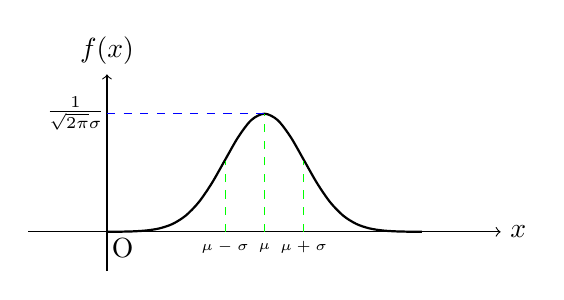
\begin{tikzpicture}
				\draw[->] (-1,0) -- (5,0) node[right] {$x$};
				\draw[->] (0,-0.5) -- (0,2) node[above] {$f(x)$};
				\draw[thick, domain=0:4, smooth, variable=\x] plot ({\x},{1.5*(2.7)^(-2*(\x-2)^(2)});
				\node at (0.2,-0.2) {O};
				\draw[dashed,blue] (0,1.5) -- (2,1.5);
				\draw[dashed,green] (1.5,0) -- (1.5,0.9);
				\draw[dashed,green] (2,0) -- (2,1.5);
				\draw[dashed,green] (2.5,0) -- (2.5,0.9);
				\node at (1.5,-0.2) {\tiny{$\mu-\sigma$}};
				\node at (2,-0.2) {\tiny{$\mu$}};
				\node at (2.5,-0.2) {\tiny{$\mu+\sigma$}};
				\node at (-0.4,1.5) {\small{$\frac{1}{\sqrt{2\pi}\sigma}$}};
			\end{tikzpicture}	
		}
		\subfigure[标准正态分布概率密度]{
			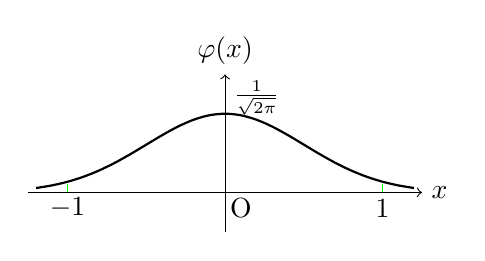
\begin{tikzpicture}
				\draw[->] (-2.5,0) -- (2.5,0) node[right] {$x$};
				\draw[->] (0,-0.5) -- (0,1.5) node[above] {$\varphi(x)$};
				\draw[thick, domain=-2.4:2.4, smooth, variable=\x] plot ({\x},{(2.71)^(-0.5*(\x)^(2)});
				\node at (0.2,-0.2) {O};
				\draw[dashed,green] (2,0) -- (2,0.137);
				\draw[dashed,green] (-2,0) -- (-2,0.137);
				\node at (-2,-0.2) {$-1$};
				\node at (2,-0.2) {$1$};
				\node at (0.4,1.2) {\small{$\frac{1}{\sqrt{2\pi}}$}};
			\end{tikzpicture}	
		}
		\caption{一般正态分布和标准正态分布概率密度函数}
		\label{figure: 一般正态分布和标准正态分布概率密度函数}
	\end{figure}
	\begin{corollary}[正态分布函数性质]
		\begin{itemize}
			\item $F(x) = P(X\leq x) = \varPhi(\dfrac{x-\mu}{\sigma})$
			\item $P(a\leq X\leq b) = \varPhi(\dfrac{b-\mu}{\sigma})-\varPhi(\dfrac{a-\mu}{\sigma})$
			\item $F(\mu-x) + F(\mu+x) = 1, aX + b\sim N(a\mu+b,a^{2}\sigma^{2})$
		\end{itemize}
	\end{corollary}
\end{definition}

\section{一维随机变量函数的分布}

\begin{definition}
	设 $X$ 是随机变量, 函数 $y = g(x)$, 以随机变量 $X$ 作为自变量的函数 $Y = g(X)$ 也是随机变量, 称为随机变量函数
	\begin{itemize}
		\item 离散型 $\to$ 离散型
		\item 连续型 $\to$ 连续型
		\item 连续型 $\to$ 离散型
	\end{itemize}
\end{definition}


\chapterimage{chap23.jpg}
\chapter{多维随机变量及其分布}

\section{$n$ 维随机变量及其分布函数}

\begin{definition}[$n$维随机变量]
	如果 $X_{1}, X_{2}, \cdots, X_{n}$ 是定义在同一个样本空间 $\Omega$ 上的 $n$ 个随机变量, 称 $(X_{1}, X_{2}, \cdots, X_{n})$ 为 $n$ 维随机向量
\end{definition}

\begin{definition}[$n$维随机变量分布函数]

	对于任意的 $n$ 个实数 $x_{1}, x_{2}, \cdots, x_{n}$, $n$ 元函数
	$$F(x_{1}, x_{2}, \cdots, x_{n}) = P\{X_{1}\leq x_{1},X_{2}\leq x_{2},\cdots,X_{n}\leq x_{n}\}$$
	
	称为 $n$ 维随机向量 $(X_{1},X_{2},\cdots,X_{n})$ 的\textbf{联合分布函数}
	
	特别的,当 $n = 2$ 时, 记 $(X,Y)$ 为 \textbf{二维随机变量} 或者 \textbf{二维随机向量}, 称 $F(x,y) = P\{X\leq x,Y\leq y\}$ 为二维随机变量 $(X,Y)$ 的联合分布函数 
	
	$$(X,Y)\sim F(x,y)\Leftrightarrow F(x,y)=P\{X\leq x,Y\leq y\}$$
\end{definition}

\begin{corollary}[二维随机变量联合分布性质]
	(1). \textcolor{blue}{单调性 (单调不减)}
	$$\forall x, y_{1}<y_{2}, F(x,y_{1})\leq F(x,y_{2})$$
	$$\forall y, x_{1}<x_{2}, F(x_{1},y)\leq F(x_{1},y)$$
	
	(2). \textcolor{blue}{右连续性}
	$$\begin{cases}
		\lim\limits_{x\to x_{0}^{+}}F(x,y) = F(x_{0}+0,y) = F(x_{0},y)\\
		\lim\limits_{y\to y_{0}^{+}}F(x,y) = F(x,y_{0}+0) = F(x,y_{0})
	\end{cases}$$
	
	(3). \textcolor{blue}{有界性}
	$$\begin{cases}
		F(-\infty,y) = F(x,-\infty) = F(-\infty,-\infty) = 0\\ 
		F(+\infty,+\infty) = 1
	\end{cases}$$
	
	(4). \textcolor{blue}{非负性}
	$\forall x_{1} < x_{2}, y_{1}<y_{2}$
	$$F(x_{1} < x \leq x_{2}, y_{1} <y\leq y_{2}) = F(x_{2},y_{2}) - F(x_{2},y_{1}) - F(x_{1},y_{2}) + F(x_{1},y_{1})\geq 0$$
\end{corollary}

\begin{definition}[边缘分布函数]
	设二维随机变量 $(X,Y)$ 的分布函数 $F(X,Y)$, 随机变量 $X$ 与 $Y$ 的分布函数 $F_{X}(x)$ 和 $F_{Y}(y)$ 分别称为随机变量关于 $(X,Y)$ 关于 $X$ 和 $Y$ 的\textbf{边缘分布函数}
	$$\begin{cases}
		F_{X}(x) = P\{X\leq x\} = P\{X\leq x,Y<+\infty\} = F(x,+\infty)\\
		F_{Y}(y) = P\{Y\leq y\} = P\{X<+\infty,Y\leq y\} = F(+\infty,y)
	\end{cases}$$
\end{definition}

\section{二维离散型随机变量}

\begin{definition}[概率分布]
	二维随机变量 $(X,Y)$ 只能取有限对值或可列无限对值 $(x_{1},y_{1}), (x_{2},y_{2}), \cdots, (x_{n},y_{n}), \cdots$, 称 $(X,Y)$ 为\textbf{二维离散型随机变量}, $(X,Y)$满足概率分布

	$$p_{ij} = P\{X = x_{i}, Y = y_{j}\} (i,j = 1,2,\cdots)$$
	
	上面的式子称为 $(X,Y)$ 的联合分布律, 记作 $(X,Y)\sim p_{ij}$, 见 $\mathbf{table: }$ \ref{table: 离散型二维随机变量概率分布}所示

	$$F(x,y)=P\{X\leq x,Y\leq y\}=\sum\limits_{i=1}^{\infty}\sum\limits_{j=1}^{\infty}p_{ij}$$
\end{definition}
\begin{table}[H]
	\centering
	\caption{离散型二维随机变量概率分布}
	\label{table: 离散型二维随机变量概率分布}
	\begin{tblr}{
			hline{1,Z} = {2pt},
			hline{2,Y} = {1pt},
			vline{2,Y} = {1pt},
			cells = {$},
			cell{1}{1} = {mode = text}
	}
		\diagbox{$X$}{$Y$}                     & y_{1}  & \cdots & y_{j}  & \cdots & P\{ X=x_{i}\} \\
		x_{1}                                  & p_{11} & \cdots & p_{1j} & \cdots & p_{1*}                             \\
		\vdots                                 & \vdots &        & \vdots &        & \vdots                             \\
		x_{i}                                  & p_{i1} & \cdots & p_{ij} & \cdots & p_{i*}                             \\
		\vdots                                 & \vdots &        & \vdots &        & \vdots                             \\
		P\{ Y=y_{j}\}                          & p_{*1} & \cdots & p_{*j} & \cdots & 1                                  \\
	\end{tblr}
	
\end{table}

\begin{definition}[边缘分布]
	$X$ \textbf{边缘分布}
	
	$$p_{i*} = P\{X = x_{i}\} = \sum\limits_{j = 1}^{\infty}P\{X = x_{i}, Y = y_{j}\} = \sum\limits_{j = 1}^{\infty}p_{ij} (i = 1,2,\cdots)$$
	
	$Y$ \textbf{边缘分布}
	
	$$p_{*j} = P\{Y = y_{j}\} = \sum\limits_{i = 1}^{\infty}P\{X = x_{i}, Y = y_{j}\} = \sum\limits_{i = 1}^{\infty}p_{ij} (j = 1,2,\cdots)$$
\end{definition}

\begin{definition}[条件分布]
	$X$ 在 $Y = y_{j}$ 下的条件分布 
	
	$$P\{X = x_{i}\big|Y = y_{j}\} = \dfrac{P\{X = x_{i}, Y = y_{j}\}}{P\{Y = y_{j}\}} = \dfrac{p_{ij}}{p_{*j}} (i = 1,2,\cdots)$$
	
	$Y$ 在 $X = x_{i}$ 下的条件分布
	
	$$P\{Y = y_{j}\big|X = x_{i}\} = \dfrac{P\{X = x_{i}, Y = y_{j}\}}{P\{X = x_{i}\}} = \dfrac{p_{ij}}{p_{i*}} (j = 1,2,\cdots)$$	
\end{definition}


\section{二维连续型随机变量}

\begin{definition}[分布函数和概率密度]
	二维随机变量 $(X,Y)$ 的分布函数 $F(X,Y)$ 可以表示为:

	$$F(x,y) = \int_{-\infty}^{x}\int_{-\infty}^{y}f(u,v)dudv, (x,y)\in\mathbb{R}^2$$
	
	其中 $f(x,y)$ 是非负可积函数, 且 $\int_{-\infty}^{+\infty}\int_{-\infty}^{+\infty}f(x,y)dxdy = 1$, 称 $(X,Y)$ 是\textbf{二维连续型随机变量}, 
	$f(x,y)$ 是随机变量 $(X,Y)$ 的\textbf{概率密度函数}, 记作 $(X,Y)\sim f(x,y)$
\end{definition}

\begin{corollary}[分布函数和概率密度性质]
	\begin{itemize}
		\item $P\{(X,Y)\in G\} = \iint\limits_{G}f(x,y)dxdy$
		\item $f(x,y)$ 在点 $(x_{0},y_{0})$ 处连续 $\Rightarrow \dfrac{\partial^2 F(x,y)}{\partial x\partial y}\big|_{(x_{0},y_{0})} = f(x_{0},y_{0})$
		\item $F(x,y)$ 连续且可导, $\dfrac{\partial^{2} F(x,y)}{\partial x\partial y} = f(x,y)$
	\end{itemize}
\end{corollary}

\begin{definition}[边缘分布函数和边缘概率密度]
	
	$(X,Y)\sim f(x,y)$, $X,Y$的边缘分布函数和边缘概率密度 
	
	\textcolor{red}{边缘分布函数}
	
	$$\begin{cases}
		F_{X}(x) = F(x,+\infty) = \int_{-\infty}^{x}\left[ \int_{-\infty}^{+\infty}f(u,v)dv\right] du\\
		F_{Y}(y) = F(+\infty,y) = \int_{-\infty}^{y}\left[ \int_{-\infty}^{+\infty}f(u,v)du\right] dv
	\end{cases}$$
	
	\textcolor{blue}{边缘概率密度}
	
	$$\begin{cases}
		f_{X}(x) = \int_{-\infty}^{+\infty}f(x,y)dy\\
		f_{Y}(y) = \int_{-\infty}^{+\infty}f(x,y)dx
	\end{cases}$$
\end{definition}

\begin{definition}[条件分布函数和条件概率密度]

	$(X,Y)\sim f(x,y)$, $X$ 在 $Y = y$ 条件下的\textbf{条件概率密度}和 $Y$ 在 $X = x$ 条件下的\textbf{条件概率密度}
	
	$$\begin{cases}
		f_{X\big|Y}(x\big|y) = \dfrac{f(x,y)}{f_{Y}(y)} = \dfrac{f(x,y)}{\int_{-\infty}^{+\infty}f(x,y)dx}\\
		f_{Y\big|X}(y\big|x) = \dfrac{f(x,y)}{f_{X}(x)} = \dfrac{f(x,y)}{\int_{-\infty}^{+\infty}f(x,y)dy}
	\end{cases}$$

	$$f(x,y) = 
	\begin{cases}
		f_{X}(x)f_{Y\big|X}(y\big|x) \\
		f_{Y}(y)f_{X\big|Y}(x\big|y) 
	\end{cases}$$
	
	$(X,Y)\sim f(x,y)$, $X$ 在 $Y = y$ 条件下的\textbf{条件分布函数}和 $Y$ 在 $X = x$ 条件下的\textbf{条件分布函数}

	$$\begin{cases}
		F_{Y\big|X}(y\big|x) = \int_{-\infty}^{y}f_{Y\big|X}(y\big|x)dy = \int_{-\infty}^{y}\dfrac{f(x,y)}{f_{X}(x)}dy\\
		F_{X\big|Y}(x\big|y) = \int_{-\infty}^{x}f_{X\big|Y}(x\big|y)dx = \int_{-\infty}^{x}\dfrac{f(x,y)}{f_{Y}(y)}dx
	\end{cases}$$
\end{definition}

\subsection{常见二维连续型随机变量分布}

\begin{definition}[二维均匀分布]
	$(X,Y)$ 在有界区域 $D$ 服从\textbf{均匀分布}, $(X,Y)$ 的概率密度 
	
	$$f(x,y) = 
	\begin{cases}
		\dfrac{1}{S_{D}} & (x,y)\in D\\
		0 & (x,y)\notin D
	\end{cases}$$
\end{definition}

\begin{definition}[二维正态分布]
	$(X,Y)$ 概率密度

	$$f(x,y) = \dfrac{1}{2\pi\sigma_{1}\sigma_{2}\sqrt{1-\rho^2}}exp\left\{-\dfrac{1}{2(1-\rho^2)}\left[ \left( \dfrac{x-\mu_{1}}{\sigma_{1}}\right)^2-2\rho\left( \dfrac{x-\mu_{1}}{\sigma_{1}}\right)\left( \dfrac{x-\mu_{2}}{\sigma_{2}}\right) +\left( \dfrac{x-\mu_{2}}{\sigma_{2}}\right)^2\right] \right\} $$
	
	其中 $\mu_{1},\mu_{2}\in\mathbb{R}, \sigma_{1},\sigma_{2} > 0, -1 < \rho <1$, 称 $(X,Y)$ 服从参数为 $\mu_{1},\mu_{2},\sigma_{1},\sigma_{2},\rho$ 的二维正态分布,
	记作 $(X,Y)\sim N(\mu_{1},\mu_{2};\sigma_{1}^2,\sigma_{2}^2;\rho)$
\end{definition}

\begin{corollary}[二维正态分布性质]
	\begin{itemize}
		\item 若 $(X_{1},X_{2}) \sim N(\mu_{1},\mu_{2};\sigma_{1}^{2},\sigma_{2}^{2};\rho)\Rightarrow X_{1}\sim N(\mu_{1},\sigma_{1}^{2}), X_{2}\sim N(\mu_{2},\sigma_{2}^{2})$  
		\item $X_{1}\sim N(\mu_{1},\sigma_{1}^{2}), X_{2}\sim N(\mu_{2},\sigma_{2}^{2})$, 且 $X_{1}, X_{2}$ 相互独立, 则 $(X_{1},X_{2})\sim N(\mu_{1},\mu_{2};\sigma_{1}^{2},\sigma_{2}^{2};0)$
		\item $(X_{1},X_{2})\sim N\Rightarrow k_{1}X_{1} + k_{2}X_{2}\sim N$
	\end{itemize}
\end{corollary}

\section{独立性}
\begin{definition}[二维随机变量独立性]
	设二维随机变量 $(X,Y)$ 的联合分布 $F(x,y)$, 边缘分布分别为 $F_{X}(x)$ 和 $F_{Y}(y)$, 如果任意实数对 $(x,y)$ 
	
	$$F(x,y) = F_{X}(x)F_{Y}(y)$$
	
	称 $X$ 和 $Y$\textbf{相互独立}
\end{definition}
\begin{definition}[$n$ 维随机变量独立性]
	设 $n$ 维随机变量 $(X_{1},X_{2},\cdots,X_{n})$ 的联合分布 $F(x_{1},x_{2},\cdots,x_{n})$, 
	边缘分布分别为 $F_{X_{1}}(x_{1}),F_{X_{2}}(x_{2}),\cdots,F_{X_{n}}(x_{n})$, 如果任意实数对 $(x_{1},x_{2},\cdots,x_{n})$
	
	$$F(x_{1},x_{2},\cdots,x_{n}) = F_{X_{1}}(x_{1})F_{X_{2}}(x_{2})\cdots F_{X_{n}}(x_{n})$$
	
	称 $X_{1},X_{2},\cdots,X_{n}$ \textbf{相互独立}
\end{definition}

\begin{corollary}[独立性性质]
	\begin{itemize}
		\item $n$ 个随机变量 $X_{1}, X_{2}, \cdots, X_{n}$ 相互独立 $\Leftrightarrow \forall x_{i}\in \mathbb{R} (i = 1,2,\cdots,n)$, 
		$n$ 个事件 $\{X_{1}\leq x_{1}\}, \{X_{2}\leq x_{2}\},\cdots,\{X_{n}\leq x_{n}\}$ 相互独立 
		\item 离散型二维随机变量 $(X,Y)$ 相互独立 $\Leftrightarrow \forall x_{i},y_{j} (i,j = 1,2,\cdots), P\{X = x_{i},Y = y_{j}\} = P\{X = x_{i}\} \cdot P\{Y = y_{j}\}$
		\item 连续型二维随机变量 $(X,Y)$ 相互独立 $\Leftrightarrow \forall x,y, f(x,y) = f_{X}(x)f_{Y}(y)$
		\item $(X_{1}, X_{2}, \cdots, X_{n})$ 相互独立, 其中任意 $k(2\leq k\leq n)$ 个随机变量相互独立
		\item $(X_{1}, X_{2}, \cdots, X_{n})$ 相互独立, $g_{1}(x), g_{2}(x), \cdots, g_{n}(x)$ 是一元连续函数, $g_{1}(X_{1}), g_{2}(X_{2}),\cdots,g_{n}(X_{n})$ 相互独立
		\item 独立的二维随机变量, 边缘分布和条件分布相等, 边缘概率密度与条件概率密度相等
	\end{itemize}
\end{corollary}


\section{多维随机变量函数的分布}
\begin{definition}[二维随机变量函数]
	设 $X,Y$ 为随机变量, $g(x,y)$ 是二元函数, 以随机变量 $X,Y$ 作为自变量的函数 $Z = g(X,Y)$ 也是随机变量, 称为\textbf{随机变量函数}
\end{definition}
\begin{theorem}[随机变量函数分布函数和概率密度]
	设 $X,Y$ 是随机变量, $f(x,y)$ 是 $(X,Y)$ 的概率密度, 
	$\begin{cases}
		U = G(X,Y)\\
		V = H(X,Y)
	\end{cases}$, 求 $U = g(X,Y)$ 和 $V = h(X,Y)$ 的分布函数和概率密度

	$$\begin{cases}
		U = G(X,Y)\\
		V = H(X,Y)
	\end{cases}\Rightarrow 
	\begin{cases}
		X = P(U,V)\\
		Y = Q(U,V)
	\end{cases}\Rightarrow
	\big|J\big| = 
	\begin{Vmatrix}
		\dfrac{\partial X}{\partial U} & \dfrac{\partial X}{\partial V}\\
		\dfrac{\partial Y}{\partial U} & \dfrac{\partial Y}{\partial V}
	\end{Vmatrix}$$

	$$F(u,v) = P\{U(X,Y)\leq u, V(X,Y)\leq v\} = \iint\limits_{D_{xy}}f(x,y)dxdy$$
	
	\begin{eqnarray*}
		F(u,v) & = & \iint\limits_{D_{xy}}f(x,y)dxdy\\
			   & = & \iint\limits_{D_{uv}}f(P(u,v),Q(u,v))\big|J\big|dudv\\
	\end{eqnarray*}

	$$f(u,v) = \dfrac{\partial^{2}F(u,v)}{\partial u \partial v} = f(P(u,v),Q(u,v))\big|J\big|$$

	$$\begin{cases}
		f_{U}(u) = \int_{-\infty}^{+\infty}f(u,v)dv = \int_{-\infty}^{+\infty}f(P(u,v),Q(u,v))\big|J\big|dv\\
		f_{V}(v) = \int_{-\infty}^{+\infty}f(u,v)du = \int_{-\infty}^{+\infty}f(P(u,v),Q(u,v))\big|J\big|du
	\end{cases}$$

	$$\begin{cases}
		F_{U}(u_{0}) = \int_{-\infty}^{u_{0}}du\int_{-\infty}^{+\infty}f(P(u,v),Q(u,v))\big|J\big|dv\\
		F_{V}(v_{0}) = \int_{-\infty}^{v_{0}}dv\int_{-\infty}^{+\infty}f(P(u,v),Q(u,v))\big|J\big|du
	\end{cases}$$
\end{theorem}

\begin{proposition}[和的分布]
	$(X,Y)\sim f(x,y)$, $Z = X + Y$, 求 $Z$ 的分布函数和概率密度
	\begin{figure}[H]
		\centering  %图片全局居中
		\subfigure[$X+Y$]{
			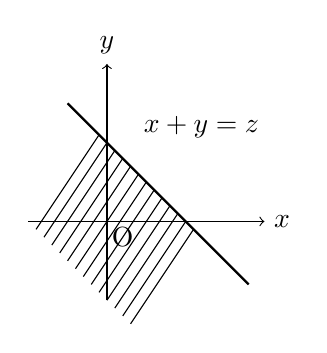
\begin{tikzpicture}
				\draw[->] (-1,0) -- (2,0) node[right] {$x$};
				\draw[->] (0,-1) -- (0,2) node[above] {$y$};
				\draw[thick, domain=-0.5:1.8, smooth, variable=\x] plot ({\x},{1-\x});
				\node at (0.2,-0.2) {O};
				\node at (1.2,1.2) {$x+y =z$};
				\foreach \i in {0,0.1,0.2,0.3,0.4,0.5,0.6,0.7,0.8,0.9,1,1.1,1.2}
				{
					\draw (\i-0.1,1.1-\i) -- (\i-0.9,-0.1-\i);
				}
			\end{tikzpicture}
		}
		\caption{和的分布}
		\label{figure: 和的分布}
	\end{figure}
	
	$$\begin{cases}
		Z = X + Y\\
		W = Y
	\end{cases}\Rightarrow
	\begin{cases}
		X = Z - W\\
		Y = W
	\end{cases}\Rightarrow \big|J\big| = 1$$
	\textbf{概率密度}
	$$f_{Z}(z) = \int_{-\infty}^{+\infty}f(z-w,w)dw$$
	\textbf{分布函数}
	$$F_{Z}(z_{0}) = \int_{-\infty}^{z_{0}}dz\int_{-\infty}^{+\infty}f(z-w,w)dw$$
\end{proposition}

\begin{proposition}[差的分布]
	$(X,Y)\sim f(x,y)$, $Z = X - Y$, 求 $Z$ 的分布函数和概率密度
	\begin{figure}[H]
		\centering  %图片全局居中
		\subfigure[$X-Y$]{
			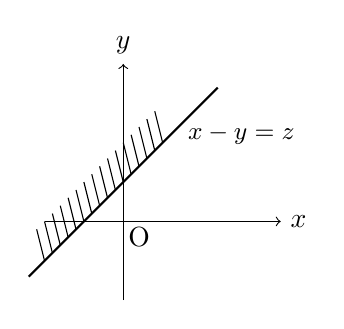
\begin{tikzpicture}
				\draw[->] (-1,0) -- (2,0) node[right] {$x$};
				\draw[->] (0,-1) -- (0,2) node[above] {$y$};
				\draw[thick, domain=-1.2:1.2, smooth, variable=\x] plot ({\x},{\x+0.5});
				\node at (0.2,-0.2) {O};
				\node at (1.5,1.1) {\small{$x-y =z$}};
				\foreach \i in {0,0.1,0.2,0.3,0.4,0.5,0.6,0.7,0.8,0.9,1,1.1,1.2,1.3,1.4,1.5}
				{
					\draw (\i-1,\i-0.5) -- (\i-1.1,\i-0.1);
				}
			\end{tikzpicture}	
		}
		\caption{差的分布}
		\label{figure: 差的分布}
	\end{figure}

	$$\begin{cases}
		Z = X - Y\\
		W = Y
	\end{cases}\Rightarrow
	\begin{cases}
		X = Z + W\\
		Y = W
	\end{cases}\Rightarrow \big|J\big| = 1$$
	\textbf{概率密度}
	$$f_{Z}(z) = \int_{-\infty}^{+\infty}f(z+w,w)dw$$
	\textbf{分布函数}
	$$F_{Z}(z_{0}) = \int_{-\infty}^{z_{0}}dz\int_{-\infty}^{+\infty}f(z+w,w)dw$$
\end{proposition}

\begin{proposition}[积的分布]
	$(X,Y)\sim f(x,y)$, $Z = XY$, 求 $Z$ 的分布函数和概率密度
	\begin{figure}[H]
		\centering  %图片全局居中
		\subfigure[$XY$]{
			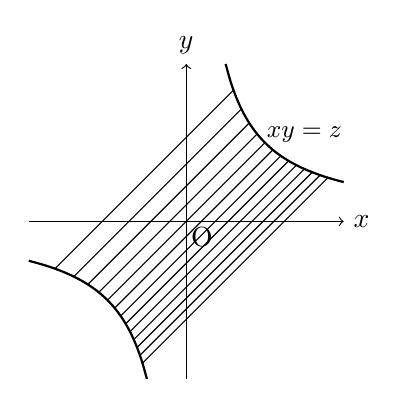
\begin{tikzpicture}
				\draw[->] (-2,0) -- (2,0) node[right] {$x$};
				\draw[->] (0,-2) -- (0,2) node[above] {$y$};
				\draw[thick, domain=0.5:2, smooth, variable=\x] plot ({\x},{1/\x});
				\draw[thick, domain=-2:-0.5, smooth, variable=\x] plot ({\x},{1/\x});
				\node at (0.2,-0.2) {O};
				\node at (1.5,1.1) {\small{$xy=z$}};
				\foreach \i in {0.6,0.7,0.8,0.9,1,1.1,1.2,1.3,1.4,1.5,1.6,1.7,1.8}
				{
					\draw (\i,1/\i) -- (-1/\i,-\i);
				}
			\end{tikzpicture}	
		}
		\caption{积的分布}
		\label{figure: 积的分布}
	\end{figure}

	$$\begin{cases}
		Z = XY\\
		W = Y
	\end{cases}\Rightarrow
	\begin{cases}
		X = \dfrac{Z}{W}\\
		Y = W
	\end{cases}\Rightarrow \big|J\big| = \big|\dfrac{1}{w}\big|$$
	\textbf{概率密度}
	$$f_{Z}(z) = \int_{-\infty}^{+\infty}f(\frac{z}{w},w)\big|\dfrac{1}{w}\big|dw$$
	\textbf{分布函数}
	$$F_{Z}(z_{0}) = \int_{-\infty}^{z_{0}}dz\int_{-\infty}^{+\infty}f(z-w,w)\big|\dfrac{1}{w}\big|dw$$
\end{proposition}
\begin{proposition}[商的分布]
	$(X,Y)\sim f(x,y)$, $Z = \dfrac{X}{Y}$, 求 $Z$ 的分布函数和概率密度

	\begin{figure}[H]
		\centering  %图片全局居中
		\subfigure[$\dfrac{X}{Y}$]{
			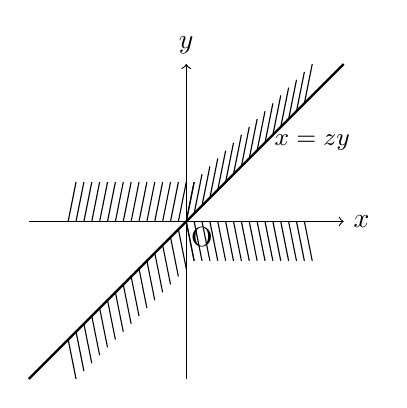
\begin{tikzpicture}
				\draw[->] (-2,0) -- (2,0) node[right] {$x$};
				\draw[->] (0,-2) -- (0,2) node[above] {$y$};
				\draw[thick, domain=-2:2, smooth, variable=\x] plot ({\x},{\x});
				\node at (0.2,-0.2) {O};
				\node at (1.6,1) {\small{$x=zy$}};
				\foreach \i in {0,0.1,0.2,0.3,0.4,0.5,0.6,0.7,0.8,0.9,1,1.1,1.2,1.3,1.4,1.5}
				{
					\draw (-\i,0) -- (-\i+0.1,0.5);
					\draw (\i,0) -- (\i+0.1,-0.5);
					\draw (\i,\i) -- (\i+0.1,\i+0.5);
					\draw (-\i,-\i) -- (-\i+0.1,-\i-0.5);
				}
			\end{tikzpicture}	
		}
		\caption{商的分布}
		\label{figure: 商的分布}
	\end{figure}
	$$\begin{cases}
		Z = \dfrac{X}{Y}\\
		W = Y
	\end{cases}\Rightarrow
	\begin{cases}
		X = ZW\\
		Y = W
	\end{cases}\Rightarrow \big|J\big| = \big|w\big|$$
	\textbf{概率密度}
	$$f_{Z}(z) = \int_{-\infty}^{+\infty}f(\frac{z}{w},w)\big|w\big|dw$$
	\textbf{分布函数}
	$$F_{Z}(z_{0}) = \int_{-\infty}^{z_{0}}dz\int_{-\infty}^{+\infty}f(z-w,w)\big|w\big|dw$$
\end{proposition}

	
\begin{proposition}[最大值和最小值的分布]
	$(X,Y)\sim f(x,y)$, $Z_{1} = \max\{X,Y\}, Z_{2} = \min\{X,Y\}$, 求 $Z_{1}, Z_{2}$ 的分布函数和概率密度
	
	$\max\{X,Y\}$ \textbf{分布函数}
	$$F_{Z_{1}}(z) = P\{Z_{1}\leq \max\{X,Y\}\} = P\{X\leq z, Y\leq z\} = F(z,z)$$
	$\max\{X,Y\}$ \textbf{概率密度}
	$$f_{Z_{1}}(z) = F'_{Z_{1}}(z)$$

	$\min\{X,Y\}$ \textbf{分布函数}
	$$F_{Z_{2}}(z) = P\{Z_{2}\leq \min\{X,Y\}\} = P\{X\leq z\} \cup P\{Y\leq z\} = F_{X}(z) + F_{Y}(z) - F(z,z)$$
	$\min\{X,Y\}$ \textbf{概率密度}
	$$f_{Z_{2}}(z) = F'_{Z_{2}}(z)$$
\end{proposition}	

\begin{corollary}[独立同分布随机变量推论]
	随机变量 $X_{1}, X_{2}, \cdots, X_{n}$ 相互独立, $Z_{1} = \max\{X_{1}, X_{2}, \cdots, X_{n}\}, Z_{2} = \min\{X_{1}, X_{2}, \cdots, X_{n}\}$, $Z_{1}, Z_{2}$ 的分布函数
	$$\begin{cases}
		F_{Z_{1}}(z) = F_{X_{1}}(z)F_{X_{2}}(z)\cdots F_{X_{n}}(z)\\
		F_{Z_{2}}(z) = 1-[1-F_{X_{1}}(z)][1-F_{X_{2}}(z)]\cdots[1-F_{X_{n}}(z)]
	\end{cases}$$

	假设随机变量 $X_{i}(i = 1, 2, \cdots, n)$ 独立同分布
	\begin{itemize}
		\item $F_{Z_{1}}(x) = [F(x)]^{n}$, $f_{Z_{1}}(x) = n[F(x)]^{n-1}f(x)$
		\item $F_{Z_{2}}(x) = 1-[1-F(x)]^{n}$, $f_{Z_{2}}(x) = nf(x)[1-F(x)]^{n-1}$
	\end{itemize}
\end{corollary}

\begin{table}[ht]
	\centering
	\caption{常见独立分布可加性}
	\label{table: 常见独立分布可加性}
	\begin{tblr}{
		hlines,
		vline{2,3},
		cells = {c,$}
	}
		X                       & Y                       & X+Y                                         \\
		B(n,p)                  & B(m,p)                  & B(n+m,p)                                    \\
		P(\lambda_{1})          & P(\lambda_{2})          & P(\lambda_{1}+\lambda_{2})                  \\
		N(\mu_{1},\sigma_{1}^2) & N(\mu_{2},\sigma_{2}^2) & N(\mu_{1}+\mu_{2},\sigma_{1}^2+\sigma_{2}^2)\\
		\chi^2(n)               & \chi^2(m)               & \chi^2(n+m)                                 \\
	\end{tblr}
\end{table}
\chapterimage{chap24.jpg}
\chapter{随机变量的数字特征}
\section{一维随机变量的数字特征}

\begin{definition}[数学期望]
	\textcolor{red}{离散型随机变量}

	$X$ 是离散型随机变量, $X$ 的分布列为 $p_{i} = P\{X = x_{i}\}(i = 1, 2, \cdots, n)$
	
	如果级数 $\sum\limits_{i = 1}^{+\infty} x_{i}p_{i}$ \textbf{绝对收敛}, 称随机变量 $X$ 的\textbf{数学期望}存在, 将其记作 $E(X)$
	
	$$E(X) = \sum\limits_{i = 1}^{+\infty}x_{i}p_{i}$$
	
	\textcolor{red}{连续型随机变量}

	$X$ 是连续型随机变量, $X$ 的概率密度为 $f(x)$
	
	如果积分 $\int_{-\infty}^{+\infty}xf(x)dx$ \textbf{绝对收敛}, 称随机变量 $X$ 的\textbf{数学期望}存在, 将其记作 $E(X)$
	
	$$E(X) = \int_{-\infty}^{+\infty}xf(x)dx$$
\end{definition}
\begin{corollary}[数学期望推论]
	\begin{itemize}
		\item $E(a) = a$, $E(E(X)) = E(X)$
		\item $E(aX \pm bY) = aE(X) \pm bE(Y)$
		\item $E\left(\sum\limits_{i = 1}^{n}a_{i}X_{i}\right) = \sum\limits_{i = 1}^{n}a_{i}E(X_{i})$
		\item $X$ 与 $Y$相互独立 $\Rightarrow E(XY) = E(X)E(Y)$ 
		\item $X_{1}, X_{2}, \cdots, X_{n}$ 相互独立
		$$\begin{cases}
			E\left(\prod\limits_{i = 1}^{n}X_{i}\right) = \prod\limits_{i = 1}^{n}E(X_{i})\\
			E\left[\prod\limits_{i = 1}^{n}g_{i}(X_{i})\right] = \prod\limits_{i = 1}^{n}E\left[g_{i}(X_{i})\right]
		\end{cases}$$
	\end{itemize}
\end{corollary}


\begin{definition}[方差和标准差]
	设 $X$ 是随机变量, 如果 $E[(X-E(X))^{2}]$ 存在, 将 $E[(X-E(X))^{2}]$ 记作 $X$ 的方差 $D(X)$ 
	
	$$D(X) = E[(X-E(X))^{2}] = E(X^{2})-[E(X)]^2$$
	
	将 $\sqrt{D(X)}$ 称为随机变量 $X$ 的\textbf{标准差}或者\textbf{均方差}, 记作 $\sigma(X)$

	随机变量 $X^{*} = \dfrac{X - E(X)}{\sqrt{D(X)}}$ 是 $X$ 的\textbf{标准化随机变量}
	$$\begin{cases}
		E(X^{*}) = 0\\
		D(X^{*}) = 1
	\end{cases}$$
	
\end{definition}

\begin{corollary}[方差和标准差推论]
	\begin{itemize}
		\item $D(X)\geq 0$, $D(X) = E(X^2) - (E(X))^{2}$
		\item $D(c)=0, c\in \mathbb{R}$
		\item $D(aX + b) = a^{2}D(X), D(X + b) = D(X)$ 
		\item $D(X\pm Y) = D(X) + D(Y) \pm 2Cov(X,Y)$
		\item $D\left(\sum\limits_{i = 1}^{n}a_{i}X_{i}\right) = \sum\limits_{i = 1}^{n}a_{i}^{2}D(X_{i}) + 2 \sum\limits_{1 \leq i < j\leq n}a_{i}a_{j} Cov(X_{i},X_{j})$
		\item $X$ 和 $Y$ 相互独立 
		$$\begin{cases}
			D(aX + bY) = a^{2}D(X) + b^{2}D(Y)\\
			D(XY) = D(X)D(Y) + D(X)[E(Y)]^{2} + D(Y)[E(X)]^{2}\geq D(X)D(Y)
		\end{cases}$$
		\item $X_{1}, X_{2}, \cdots,X_{n}$ 相互独立 
		$$\begin{cases}
			D\left(\sum\limits_{i = 1}^{n}a_{i}X_{i}\right) = \sum\limits_{i = 1}^{n}a_{i}^{2}D(X_{i})\\
			D\left(\sum\limits_{i = 1}^{n}g_{i}(X_{i})\right) = \sum\limits_{i = 1}^{n}D\left[g_{i}(X_{i})\right]
		\end{cases}$$
		\item $\forall c\in \mathbb{R}, D(X) \leq E\left[(X-c)^{2}\right]$
	\end{itemize}
\end{corollary}


\section{二维随机变量的数字特征}

\begin{definition}[数学期望]
设 $X,Y$ 为随机变量, $g(X,Y)$ 为 $X,Y$ 的函数 ( $g$ 是连续函数)

\textcolor{red}{离散型随机变量}

	$$p_{ij} = P\{X = x_{i},Y = y_{j}\}(i,j = 1,2,\cdots)$$

	级数 $\sum\limits_{i}^{m}\sum\limits_{j}^{n}g(x_{i},y_{j})p_{ij}$ \textbf{绝对收敛} 

	$$E[g(X,Y)] = \sum\limits_{i}^{m}\sum\limits_{j}^{n} g(x_{i},y_{j})p_{ij}$$

\textcolor{red}{连续型随机变量}

	$(X,Y)$ 概率密度为 $f(x,y)$, 积分 $\int_{-\infty}^{+\infty}\int_{-\infty}^{+\infty}f(x,y)dxdy$ \textbf{绝对收敛}

	$$E[g(X,Y)] = \int_{-\infty}^{+\infty}\int_{-\infty}^{+\infty}f(x,y)dxdy$$
\end{definition}


\begin{definition}[协方差与相关系数]
	随机变量 $X$ 与 $Y$ 的方差存在且 $D(X) > 0, D(Y) > 0$, 定义随机变量 $X,Y$ 的协方差 $Cov(X,Y)$ 

	$$Cov(X,Y) = E[(X-E(X))(Y-E(Y))] = E(XY) - E(X)E(Y)$$
	
	$\rho_{XY} = \dfrac{Cov(X,Y)}{\sqrt{DX}\sqrt{DY}}$ 定义为随机变量 $X,Y$ 的\textbf{相关系数}
\end{definition}
\begin{corollary}[协方差和相关系数推论]
	\begin{itemize}
		\item $Cov(X,Y) = Cov(Y,X), Cov(X,X) = D(X), \rho_{XX} = 1$
		\item $Cov(aX + b,Y) = aCov(X,Y), Cov(X_{1} + X_{2},Y) = Cov(X_{1},Y) + Cov(X_{2},Y)$
		\item $\rho_{XY} = 0\Rightarrow X,Y$ \textbf{不相关}
		\item $\rho_{XY}\neq 0\Rightarrow X,Y$ \textbf{相关}
	\end{itemize}
\end{corollary}

\section{独立性与相关性判定、切比雪夫不等式}
\begin{corollary}[独立性与相关性判定]
	随机变量 $X,Y$ 相互独立充要条件
	$$\begin{cases}
		f(x,y) = f_{X}(x)\cdot f_{Y}(y)\\
		P\{X = x_{i},Y = y_{i}\} = P\{X = x_{i}\}\cdot P\{Y = y_{i}\}
	\end{cases}$$

	随机变量 $X,Y$ 不相关充要条件 $\rho_{XY} = 0$

	$$\rho_{XY} = 0\Leftrightarrow Cov(X,Y) = 0\Leftrightarrow E(XY) = E(X)\cdot E(Y)\Leftrightarrow D(X \pm Y) = D(X) + D(Y)$$
\end{corollary}


\begin{definition}[切比雪夫不等式]
	随机变量 $X$ 的期望 $E(X)$ 和方差 $D(X)$ 都存在
	$$\begin{cases}
		\forall \varepsilon > 0, P\{|X - E(X)|\leq \varepsilon\} \geq \dfrac{D(X)}{\varepsilon^{2}}\\
		\forall \varepsilon > 0, P\{|X - E(X)|\geq \varepsilon\} \leq 1- \dfrac{D(X)}{\varepsilon^{2}}
	\end{cases}$$
\end{definition}
\begin{table}[ht]
	\centering
	\caption{常用分布表}
	\label{table: 常用分布表}
	\begin{tblr}{
		hlines = {1pt},
		hline{1,Z} = {2pt},
		vline{2-Y} = {1pt},
		cells = {c}
	}
		$\text{名称}$                                    & $\text{概率分布}$                                                                    & $\text{均值}$            & $\text{方差}$                      & $\text{参数范围}$                       \\
		$\text{两点分布}$                                & {$P(X=k)=p^kq^{1-k}$\\ $(k=0,1)$}                                                   & $p$                      & $pq$                              & {$0<p<1$\\ $q=1-p$}                     \\
		{$\text{二项分布}$\\ $B(n,p)$}                   & {$P(X=k)=C_{n}^{k}p^kq^{n-k}$ \\ $(k=0,1,\cdots,n)$}                                & $np$                     & $npq$                             & {$0<p<1$ \\ $q=1-p$\\ $n\in N$}         \\
		{$\text{泊松分布}$\\ $P(\lambda$)}               & {$P(X=k)=\dfrac{\lambda^k}{k!}e^{-\lambda}$ \\ $(k=0,1,2,\cdots)$}                  & $\lambda$                & $\lambda$                         & $\lambda>0$                             \\
		{$\text{超几何分布}$\\ $H(n,N,M)$}               & {$P(X=k)=\dfrac{C_{N-M}^{n-k}C_{M}^{k}}{C_{N}^{n}}$\\ $(k=0,1,\cdots\,\min\{M,n\})$} & $\dfrac{nM}{N}$          & $\dfrac{n(N-n)(N-M)M}{N^2(N-1)}$  & {$n,N,M\in N$\\ $n\leq N,M\leq N$}      \\
		{$\text{几何分布}$\\ $G(p)$}                     & {$P(X=k)=(1-p)^{k-1}p$\\ $(k=1,2,\cdots)$}                                          & $\dfrac{1}{p}$           & $\dfrac{1-p}{p^2}$                & {$0<p<1$\\ $q=1-p$}                     \\
		{$\text{均匀分布}$\\ $U(a,b)$}                   & $f(x)=\dfrac{1}{b-a}(a\leq x\leq b)$                                                 & $\dfrac{a+b}{2}$         & $\dfrac{(b-a)^3}{12}$             &  \\
		{$\text{指数分布}$\\ $E(\lambda)$}               & $f(x)=\lambda e^{-\lambda x}(x>0)$                                                  & $\dfrac{1}{\lambda}$     & $\dfrac{1}{\lambda^2}$            & $\lambda>0$                             \\
		{$\text{正态分布}$\\ $N(\mu,\sigma^2)$}          & $f(x)=\dfrac{1}{\sqrt{2\pi\sigma}}e^{-\frac{(x-\mu)^2}{2\sigma^2}}$                & $\mu$                    & $\sigma^2$                        & $\sigma>0$                              \\
		{$\Gamma\text{分布}$ \\ $\Gamma(\alpha,\beta)$} & $f(x)=\dfrac{\beta^{\alpha}}{\Gamma(\alpha)}x^{\alpha-1}e^{-\beta x}(x>0)$           & $\dfrac{\alpha}{\beta}$ & $\dfrac{\alpha}{\beta^2}$          & {$\alpha>0$\\ $\beta>0$}                \\
	\end{tblr}
\end{table}
\chapterimage{chap25.jpg}
\chapter{大数定理和中心极限定理}

\section{依概率收敛}

\begin{definition}[依概率收敛]
	设随机变量 $X$ 与随机变量序列 $\{X_{n}\}(n = 1,2,3,\cdots,n)$
	
	$$\begin{cases}
		\forall \varepsilon > 0, \lim\limits_{n\Rightarrow \infty}P\{|X_{n}-X|\geq \varepsilon\} = 0\\
		\forall \varepsilon > 0, \lim\limits_{n\Rightarrow \infty}P\{|X_{n}-X|< \varepsilon\} = 1
	\end{cases}$$
	
	称随机变量序列 $\{X_{n}\}$ \textbf{依概率收敛于随机变量} $X$, 记作 
	$$\lim\limits_{n\Rightarrow \infty} X_{n} = X(P)\ or\ X_{n}\stackrel{P}{\longrightarrow}X(n\Rightarrow \infty)$$
\end{definition}

\section{大数定理}

\begin{theorem}[切比雪夫大数定理]
	假设 $\{X_{n}\}(n = 1,2,\cdots, n)$ 是相互独立的随机变量序列, 如果方差 $D(X_{i})$ 存在且一致有上界, $\forall i\geq 1,\ s.t.\ D(X_{i})\leq C, C\in \mathbb{R}$,
	$\{X_{n}\}$ 服从大数定理
	$$\dfrac{1}{n}\sum\limits_{i = 1}^{n}X_{i} \stackrel{P}{\longrightarrow} \dfrac{1}{n}\sum\limits_{i=1}^{n}E(X_{i})$$
\end{theorem}

\begin{theorem}[伯努利大数定理]
	假设 $\mu_{n}$ 是 $n$ 重伯努利试验中事件 $A$ 发生的次数, 在每次试验中事件 $A$ 发生的概率为 $p(0<p<1)$, $\dfrac{\mu_{n}}{n}\stackrel{P}{\longrightarrow}p$
	$$\forall \varepsilon > 0,\lim\limits_{n\Rightarrow \infty}P\{\big|\dfrac{\mu_{n}}{n} - p\big| < \varepsilon\} = 1$$
\end{theorem}

\begin{theorem}[辛钦大数定理]
	假设 $\{X_{n}\}$ 是独立同分布的随机变量序列, 如果 $E(X_{i}) = \mu(i = 1,2,\cdots,n)$ 存在, $\dfrac{1}{n}\sum\limits_{i=1}^{n}X_{i}\stackrel{P}{\longrightarrow}\mu$
	$$\forall \varepsilon > 0,\lim\limits_{n\Rightarrow \infty}P\{\big|\dfrac{1}{n}\sum\limits_{i=1}^{n}X_{i}-\mu\big| < \varepsilon\} = 1$$
\end{theorem}

\section{中心极限定理}

\href{https://www.bilibili.com/video/BV1gh4y1W7ag/?spm_id_from=333.999.list.card_archive.click}{中心极限定理}

\href{https://www.bilibili.com/video/BV1wu411W7uU/?spm_id_from=333.999.list.card_archive.click}{正态分布}

\begin{theorem}[列维-林德伯格定理]
	假设 $\{X_{n}\}$ 是独立同分布的随机变量序列, 如果 $E(X_{i}) = \mu, D(X_{i}) = \sigma^2 > 0(i = 1,2,\cdots,n)$
	$$\forall x \in \mathbb{R}, \lim\limits_{n\Rightarrow \infty}P\{\dfrac{\sum\limits_{i=1}^{n}X_{i}-n\mu}{\sqrt{n\sigma}}<x\} = \dfrac{1}{\sqrt{2\pi}}\int_{-\infty}^{x}e^{-\frac{t^2}{2}}dt=\varPhi(x)$$
\end{theorem}
\begin{corollary}[中心极限定理推论]
	\begin{itemize}
		\item $\sum\limits_{i = 1}^{n}X_{i}\sim N(n\mu,n\sigma^2)$
		\item $P\{a<\sum\limits_{i=1}^{n}X_{i}<b\}\approx\varPhi(\dfrac{b-n\mu}{\sqrt{n}\sigma})-\varPhi(\dfrac{a-n\mu}{\sqrt{n}\sigma})$
	\end{itemize}
\end{corollary}

\begin{theorem}[棣莫弗-拉普拉斯定理]
	假设随机变量 $Y_{n}\sim B(n,p)(0 < p < 1, n\geq 1)$
	$$\forall x\in \mathbb{R}, \lim\limits_{n\Rightarrow \infty}P\{\dfrac{Y_{n}-np}{\sqrt{np(1-p)}}<x\}=\dfrac{1}{\sqrt{2\pi}}\int_{-\infty}^{x}e^{-\frac{t^2}{2}}dt = \varPhi(x)$$
\end{theorem}

\chapterimage{chap26.jpg}
\chapter{数理统计}
\section{总体和样本}
\begin{definition}[统计概念和统计量]
	\begin{itemize}
		\item \textbf{总体}: 研究对象的全体称为总体
		\item \textbf{样本}: $n$ 个相互独立且与总体具有相同概率分布的随机变量 $X_{1}, X_{2}, \cdots, X_{n}$ 所组成的整体 $(X_{1}, X_{2}, \cdots, X_{n})$ 
		称为来自总体 $X$, 容量为 $n$ 的一个\textbf{简单随机样本}, 一次抽样结果的具体的 $n$ 个数值 $(x_{1},x_{2},\cdots,x_{n})$ 称为样本 $(X_{1},X_{2},\cdots,X_{n})$ 的一个观测值
	\end{itemize}
\end{definition}

\begin{definition}[样本分布]
	假设总体的分布函数 $F(x)$, 概率密度函数 $f(x)$, 样本 $(X_{1},X_{2},\cdots,X_{n})$ 的分布函数和概率密度
	\begin{itemize}
		\item 离散型 $P\{X_{1} = x_{1}, X_{2} = x_{2}, \cdots, X_{n} = x_{n}\} = \prod\limits_{i = 1}^{n}P\{X_{i} = x_{i}\}$
		\item 连续型 
		$$\begin{cases}
			F(x_{1},x_{2},\cdots,x_{n}) = \prod\limits_{i = 1}^{n}F(x_{i})\\
			f(x_{1},x_{2},\cdots,x_{n}) = \prod\limits_{i = 1}^{n}f(x_{i})
		\end{cases}$$
	\end{itemize}
\end{definition}

\section{统计量及其分布}
\begin{definition}
	设 $X_{1},X_{2},\cdots,X_{n}$ 是来自总体 $X$ 的一个样本,
	$g(x_{1}, x_{2}, \cdots, x_{n})$ 是 $n$ 元函数, 如果函数 $g$ 中不含任何参数, 称 $g(X_{1},X_{2},\cdots,X_{n})$ 是样本 $X_{1},X_{2},\cdots,X_{n}$ 的一个\textbf{统计量}
\end{definition}

\begin{definition}[样本数字特征]
	\begin{itemize}
		\item \textbf{样本均值} $\overline{X} = \dfrac{1}{n}\sum\limits_{i = 1}^{n}X_{i}$
		\item \textbf{样本方差} $S^{2} =\dfrac{1}{n-1}\sum\limits_{i = 1}^{n}(X_{i}-\overline{X})^2$
		\item \textbf{样本标准差} $S = \sqrt{\dfrac{1}{n-1}\sum\limits_{i = 1}^{n}(X_{i} - \overline{X})^{2}}$
		\item \textbf{样本} $k$ \textbf{阶原点矩}  $A_{k} = \dfrac{1}{n}\sum\limits_{i = 1}^{n}X_{i}^{k} (k = 1,2,\cdots)$
		\item \textbf{样本} $k$\textbf{阶中心矩} $B_{k} = \dfrac{1}{n}\sum\limits_{i = 1}^{n}(X_{i}-\overline{X})^{k} (k = 2, 3, \cdots)$
	\end{itemize}
\end{definition}

\begin{definition}[顺序统计量]
	将样本 $X_{1}, X_{2}, \cdots, X_{n}$ 的 $n$ 个观测值\textbf{从小到大}顺序排序 
	$$X_{(1)} \leq X_{(2)} \leq \cdots \leq X_{(n)}\leq$$
	
	随机变量 $X_{(k)}$ 称作第 $k$ 顺序统计量, $X_{(1)}$ 为最小顺序统计量, $X_{(n)}$为最大顺序统计量

	$$\begin{cases}
		X_{(1)} = \min\{X_{1},X_{2},\cdots,X_{n}\}\\
		X_{(n)} = \max\{X_{1},X_{2},\cdots,X_{n}\}
	\end{cases}$$
\end{definition}
\begin{corollary}[统计量(数字特征)性质]
	假设总体期望 $E(X)=\mu$, 总体方差为 $D(X) = \sigma^{2}$, $X_{1},X_{2},\cdots,X_{n}$ 是取自总体的一个样本, $\overline{X},S^{2}$ 分别为样本的均值和方差 
	\begin{itemize}
		\item $E(X_{i}) = \mu$
		\item $D(X_{i}) = \sigma^{2}$
		\item $E(\overline{X}) = E(\dfrac{X_{1}+X_{2}+\cdots+X_{n}}{n}) = E(X) = \mu$
		\item $D(\overline{X}) = D(\dfrac{X_{1}+X_{2}+\cdots+X_{n}}{n}) = \dfrac{1}{n}\sigma^{2}$
		\item $E(S^{2}) = D(X) = \sigma^{2}$
	\end{itemize}
\end{corollary}
\section{三大分布}
\begin{definition}[$\chi^{2}$ 分布]

	随机变量 $X_{1},X_{2},\cdots,X_{n}$ 相互独立, 且都服从标准正态分布, 随机变量 $X = \sum\limits_{i = 1}^{n}X_{i}^2$ 
	服从自由度为 $n$ 的卡方分布 $\chi^2(n)$, 记作 $X\sim \chi^2(n)$
	
	上 $\alpha$ 分位数: 对于给定的 $\alpha (0 < \alpha < 1)$, 称满足

	$$P\{\chi^{2} > \chi_{\alpha}^{2}(n)\} = \int_{\chi_{\alpha}^{2}(n)}^{+\infty}f(x)dx = \alpha$$
	
	的 $\chi_{\alpha}^{2}(n)$ 为 $\chi^2(n)$ 分布的上 $\alpha$ 分位数
	\begin{itemize}
		\item $X_{1}\sim \chi^{2}(n_{1}), X_{2}\sim \chi^{2}(n_{2}), X_{1},X_{2}$ 相互独立, $X_{1} + X_{2}\sim \chi^{2}(n_{1}+n_{2})$
		\item $X\sim \chi^2(n)\Rightarrow E(X) = n, D(X) = 2n$
	\end{itemize}
\end{definition}
\begin{figure}[H]
	\centering  %图片全局居中
	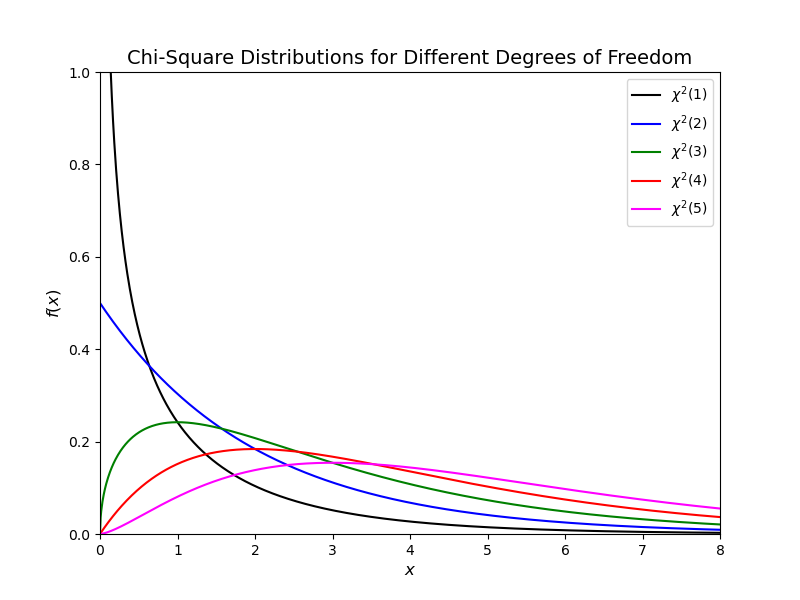
\includegraphics[width=0.7\textwidth]{"figure/Note/卡方分布.png"}
	\caption{卡方分布}
	\label{fig:卡方分布}
\end{figure}
\begin{definition}[$t$ 分布]

	随机变量 $X\sim N(0,1), Y\sim \chi^{2}(n), X, Y$ 相互独立, 随机变量 $t = \dfrac{X}{\sqrt{Y/n}}$ 服从自由度为 $n$ 的 $t$ 分布, 记作 $t\sim t(n)$
	
	上 $\alpha$ 分位数: 对于给定的 $\alpha (0 < \alpha < 1)$, 称满足

	$$P\{t > t_{\alpha}(n)\} = \alpha$$
	
	的 $t_{\alpha}(n)$ 为 $t$ 分布的上 $\alpha$ 分位数
	\begin{itemize}
		\item $t$ 分布概率密度关于 $x = 0$ 对称 $\Rightarrow E(t) = 0$
		\item $P\{t > - t_{\alpha}(n)\} = P\{t > t_{1-\alpha}(n)\} \Rightarrow t_{1-\alpha}(n) = -t_{\alpha}(n)$
	\end{itemize}
\end{definition}

\begin{figure}[H]
	\centering  %图片全局居中
	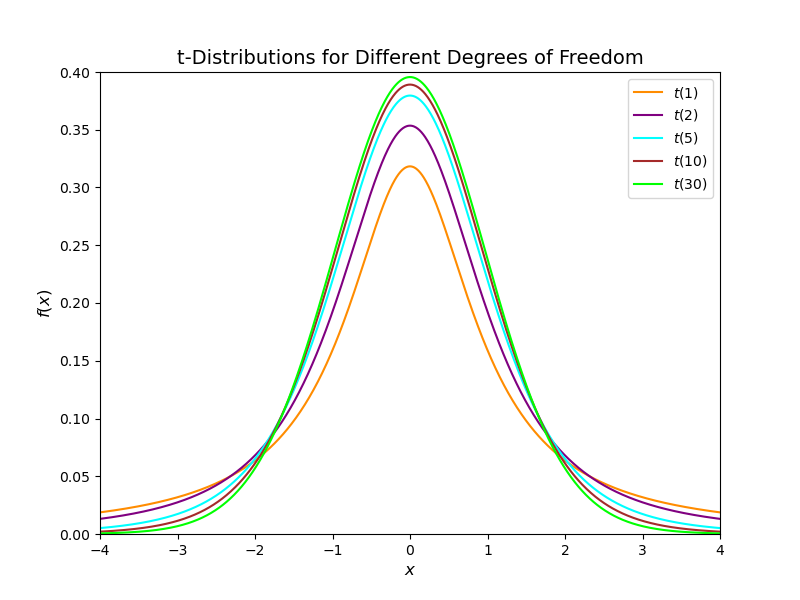
\includegraphics[width=0.7\textwidth]{"figure/Note/t分布.png"}
	\caption{ $t$ 分布}
	\label{fig: $t$ 分布}
\end{figure}

\begin{definition}[$F$ 分布]

	随机变量 $X\sim \chi^2(n_{1}), Y\sim \chi^2(n_{2})$, 且 $X,Y$ 相互独立,随机变量 $F = \dfrac{X/n_{1}}{Y/n_{2}}$ 
	服从自由度为 $(n_{1},n_{2})$ 的 $F$ 分布, 记作 $F\sim F(n_{1},n_{2})$
	
	\begin{itemize}
		\item $F\sim F(n_{1},n_{2})\Rightarrow \dfrac{1}{F}\sim F(n_{2},n_{1})$
		\item $F_{1-\alpha}(n_{1},n_{2})=\dfrac{1}{F_{\alpha}(n_{2},n_{1})}$
		\item $t\sim t(n)\Rightarrow t^{2}\sim F(1,n)$
	\end{itemize}
\end{definition}

\begin{figure}[H]
	\centering  %图片全局居中
	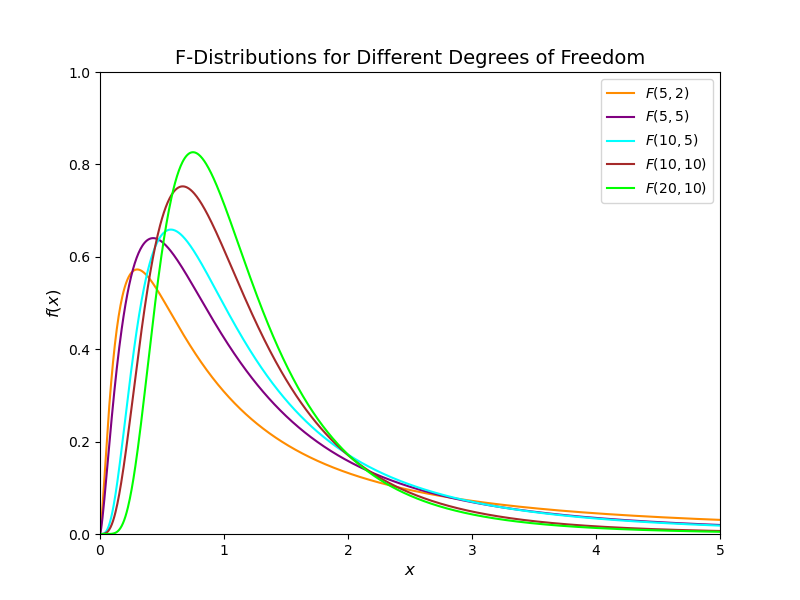
\includegraphics[width=0.7\textwidth]{"figure/Note/F分布.png"}
	\caption{ $F$ 分布}
	\label{fig: $F$ 分布}
\end{figure}

\begin{corollary}[正态总体推论]
	
	设 $X_{1}, X_{2}, \cdots, X_{n}$ 是来自正态总体 $N(\mu,\sigma^{2})$ 的一个样本, $\overline{X}, S^2$ 分别是样本的均值和方差
	\begin{itemize}
		\item $\overline{X}\sim N(\mu,\dfrac{\sigma^2}{n})\Rightarrow \dfrac{\overline{X}-\mu}{\dfrac{\sigma}{\sqrt{n}}}=\dfrac{\sqrt{n}(\overline{X}-\mu)}{\sigma}\sim N(0,1)$
		\item $\dfrac{1}{\sigma^{2}}\sum\limits_{i=1}^{n}(X_{i}-\mu)^{2}\sim \chi^{2}(n)$
		\item $\dfrac{(n-1)S^2}{\sigma^2}=\sum\limits_{i=1}^{n}(\dfrac{X_{i}-\overline{X}}{\sigma})^2\sim \chi^2(n-1)$
		\item $\overline{X}$ 和 $S^{2}$ 相互独立 $\Rightarrow \dfrac{\sqrt{n}(\overline{X}-\mu)}{S}\sim t(n-1)$
		\item $\sigma$ 未知时, $\dfrac{n(\overline{X}-\mu)^2}{S^2}\sim F(1,n-1)$
	\end{itemize}
\end{corollary}


\section{参数的点估计}
\begin{definition}[参数点估计]
	设总体 $X$ 的分布函数 $F(x;\theta)$, 其中 $\theta$ 是一个未知参数, $X_{1},X_{2},\cdots,X_{n}$ 是来自总体的一个样本,
	由样本构造一个适当的统计量 $\hat{\theta}(X_{1},X_{2},\cdots,X_{n})$ 作为参数 $\theta$ 的估计, 称统计量 $\hat{\theta}$ 为参数 $\theta$ 的估计量
\end{definition}

\begin{definition}[矩估计]
	设总体分布中有 $k$ 个未知的参数 $\theta_{1},\theta_{2},\cdots,\theta_{k}$, 来自总体 $X$ 的一组样本 $X_{1},X_{2},\cdots,X_{n}$, 
	如果 $X$ 的原点矩 $E(X^{l})(l = 1, 2, \cdots, k)$ 存在, 样本原点矩 $\dfrac{1}{n}\sum\limits_{i=1}^{n}X_{i}^{l}$ 可作为 $E(X^{l})$ 的估计
\end{definition}

\begin{definition}[最大似然估计]
	对未知参数 $\theta$ 进行估计, 在该参数可能的取值范围 $I$ 中选取, 使用使样本观测值 $x_{1},x_{2},\cdots,x_{n}$ 最大的参数 $\hat{\theta}$ 作为参数 $\theta$ 的估计值
	
	似然函数 
	$$\begin{cases}
		L(\theta) = L(x_{1},x_{2},\cdots,x_{n};\theta)\\
		L(\theta) = \prod\limits_{i=1}^{n}f(x_{i};\theta)
	\end{cases}$$
	
	$$\exists \hat{\theta}\in I,\ s.t.\ L(x_{1},x_{2},\cdots,x_{n},\hat{\theta}) = \max_{\theta\in I}L(x_{1},x_{2},\cdots,x_{n},\theta)$$
\end{definition}

\begin{corollary}[估计量评价标准]
	\begin{itemize}
		\item \textbf{无偏性}: $E(\hat{\theta}) = \theta$
		\item \textbf{有效性}: $D(\hat{\theta})$ 最小
		\item \textbf{一致性}: $\forall \varepsilon > 0, \lim\limits_{n\Rightarrow \infty}P\{|\hat{\theta}-\theta|<\varepsilon\} = 1$
	\end{itemize}
\end{corollary}

\section{参数的区间估计}

\begin{definition}[区间估计和置信区间]
	设 $\theta$ 是总体 $X$ 的一个未知参数, 对于给定的 $\alpha(0 < \alpha < 1)$, 如果由样本 $X_{1},X_{2},\cdots,X_{n}$ 确定的两个统计量 
	$\hat{\theta_{1}} = \hat{\theta_{1}}(X_{1},X_{2},\cdots,X_{n})$ 和 $\hat{\theta_{2}} = \hat{\theta_{2}}(X_{1},X_{2},\cdots,X_{n})$ 满足 
	$$P\{\hat{\theta_{1}}(X_{1},X_{2},\cdots,X_{n}) < \theta < \hat{\theta_{2}}(X_{1},X_{2},\cdots,X_{n})\} = 1-\alpha$$
	
	则称随机区间 $(\hat{\theta_{1}},\hat{\theta_{2}})$ 是 $\theta$ 的置信度为 $1-\alpha$ 的 \textbf{置信区间},
	$\hat{\theta_{1}}$ 和 $\hat{\theta_{2}}$ 分别称为 \textbf{置信上限}和\textbf{置信下限}, $1-\alpha$ 为置信水平, $\alpha$ 为\textbf{显著性水平}
\end{definition}

\begin{table}[ht]
	\centering
	\caption{正态总体的置信区间}
	\label{table: 正态总体的置信区间}
	\begin{tblr}{
		hline{1,Z} = {2pt},
		hline{2-Y} = {1pt},
		vline{2-Y} = {1pt},
		cells = {c,$}
	}
		\text{待估参数} & \text{其他参数}     & \text{枢轴量分布}                                                                  & \text{置信区间}                                                                                                 \\
		\mu            & \sigma^2\text{已知} & Z=\dfrac{\overline{X}-\mu}{\sigma/\sqrt{n}}\sim N(0,1)                            & \left( \overline{X}-\dfrac{\sigma}{\sqrt{n}}z_{\alpha/2},\overline{X}+\dfrac{\sigma}{\sqrt{n}}z_{\alpha/2}\right) \\
		\mu            & \sigma^2\text{未知} & t=\dfrac{\overline{X}-\mu}{S/\sqrt{n}}\sim t(n-1)                                 & \left( \overline{X}-\dfrac{S}{\sqrt{n}}t_{\alpha/2}(n-1),\overline{X}+\dfrac{S}{\sqrt{n}}t_{\alpha/2}(n-1)\right) \\
		\sigma^{2}     & \mu\text{已知}      & \chi^{2}=\dfrac{\sum\limits_{i=1}^{n}(X_{i}-\mu)^{2}}{\sigma^{2}}\sim \chi^{2}(n) & \left( \dfrac{\sum\limits_{i=1}^{n}(X_{i}-\mu)^{2}}{\chi_{\alpha/2}(n)},\dfrac{\sum\limits_{i=1}^{n}(X_{i}-\mu)^{2}}{\chi_{1-\alpha/2}(n)}\right) \\
		\sigma^{2}     & \mu\text{未知}      & \chi^{2}=\dfrac{(n-1)S^{2}}{\sigma^{2}}\sim \chi^{2}(n-1)                               & \left( \dfrac{(n-1)S^{2}}{\chi_{\alpha/2}^{2}(n)},\dfrac{(n-1)S^{2}}{\chi_{1-\alpha/2}^{2}(n)}\right) \\
	\end{tblr}
\end{table}
\section{假设检验}

\begin{definition}[统计性检验]
	\begin{itemize}
		\item $H_{0}$: 虚无假设
		\item $H_{1}$: 备择假设
	\end{itemize}
\end{definition}
\begin{definition}[两类错误]
	\begin{itemize}
		\item \textbf{第一类错误}: 虚无假设 $H_{0}$ 为真, 但拒绝了 $H_{0}$, 误认为备择假设 $H_{1}$ 为真, 犯第一类错误概率 $\alpha = P\{R(H_{0})\big| T(H_{0})\}$
		\item \textbf{第二类错误}: 备择假设 $H_{1}$ 为真, 但接受了 $H_{0}$, 误认为虚无假设 $H_{0}$ 为真, 犯第二类错误概率 $\beta = P\{A(H_{0})\big| T(H_{1})\}$
	\end{itemize}
\end{definition}
\begin{corollary}[正态总体下的六大检查和拒绝域]
	\begin{itemize}
		\item $\sigma^{2}$ 已知,$\mu$ 未知, $H_{0}:\ \mu = \mu_{0}, H_{1}:\ \mu \neq \mu_{0}$
		$$\mu_{r}\in (-\infty,\mu_{0}-\frac{\sigma}{\sqrt{n}}z_{\frac{\alpha}{2}})\cup (\mu_{0}+\frac{\sigma}{\sqrt{n}}z_{\frac{\alpha}{2}},+\infty)$$
		
		\item $\sigma^{2}$ 未知, $\mu$ 未知, $H_{0}:\ \mu = \mu_{0}, H_{1}:\ \mu\neq \mu_{0}$
		$$\mu_{r}\in (-\infty,\mu_{0}-\frac{S}{\sqrt{n}}t_{\frac{\alpha}{2}}(n-1))\cup (\mu_{0}+\frac{S}{\sqrt{n}}t_{\frac{\alpha}{2}}(n-1),+\infty)$$
		
		\item $\sigma^{2}$ 已知, $\mu$ 未知, $H_{0}:\ \mu\leq \mu_{0}, H_{1}:\ \mu > \mu_{0}$
		$$\mu_{r}\in (\mu_{0} + \frac{\sigma}{\sqrt{n}}z_{\alpha},+\infty)$$

		\item $\sigma^{2}$ 已知, $\mu$ 未知, $H_{0}:\ \mu\geq \mu_{0}, H_{1}:\ \mu < \mu_{0}$
		$$\mu_{r}\in (-\infty,\mu_{0}-\frac{\sigma}{\sqrt{n}}z_{\alpha})$$

		\item $\sigma^{2}$ 未知, $\mu$ 未知, $H_{0}:\ \mu\leq \mu_{0}, H_{1}:\ \mu> \mu_{0}$
		$$\mu_{r}\in (\mu_{0} + \frac{S}{\sqrt{n}}t_{\alpha}(n-1),+\infty)$$

		\item $\sigma^{2}$ 未知, $\mu$ 未知, $H_{0}:\ \mu\geq \mu_{0}, H_{1}:\ \mu< \mu_{0}$
		$$\mu_{r}\in (-\infty,\mu_{0}-\frac{S}{\sqrt{n}}t_{\alpha}(n-1))$$
	\end{itemize}
\end{corollary}